Below we introduce five additional notable 3-periodic Poncelet families interscribed between a pair of concentric, axis-parallel (CAP) ellipses. As before, the Cayley condition \cref{eqn:n3-cayley} will be used to constrain the ellipse pair. 

\begin{figure}
    \centering
    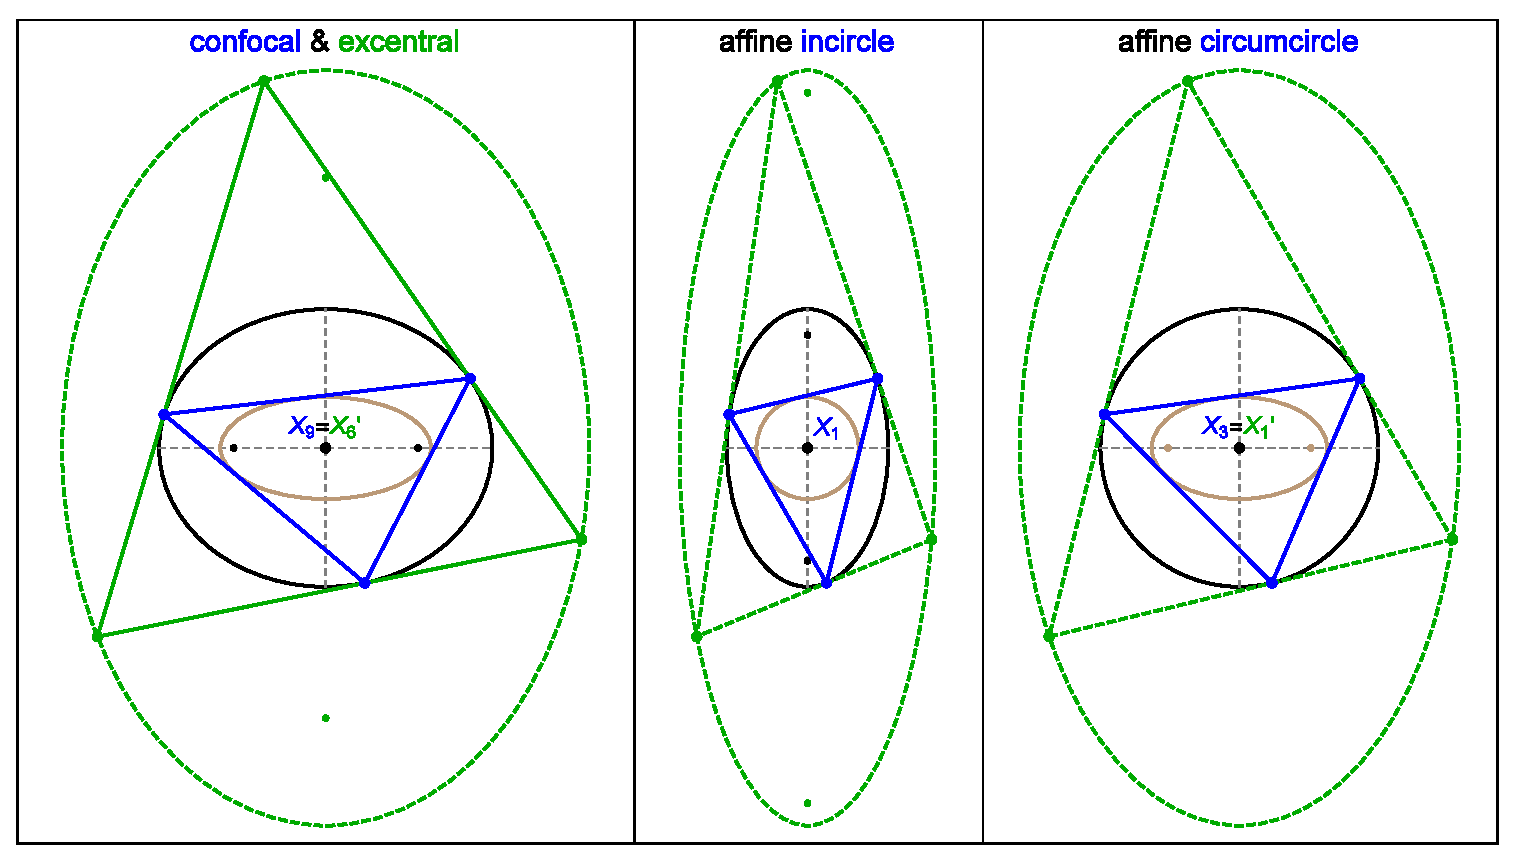
\includegraphics[width=\textwidth]{pics_03_110_n3_affine.eps}
    \caption{\textbf{Left:} billiard 3-periodic (blue) and its excentral triangle (green). The former conserves the sum of its cosines. The latter is inscribed in an ellipse (dashed green) and conserves the product of its cosines. \textbf{Middle:} Affine image of confocal family which sends caustic (brown) to a circle. This family also conserves the sum of cosines, equal to that conserved by its confocal pre-image. \textbf{Right:} Affine image of confocal family which sends billiard ellipse (black) to a circle. This family also conserves the product of cosines, equal to that conserved by the excentral family of its pre-image. \href{https://youtu.be/HjBZdrR3Azs}{Video}}
    \label{fig:03-n3-affine}
\end{figure}

\subsection{Excentral Family}

This is the Ponceletian family of excentral triangles to billiard 3-periodics. If the axes of its caustic are $a,b$, this family is inscribed in an ellipse with $a',b'$ given in \cref{thm:03-incenter-excenter}; see \cref{fig:03-n3-affine}(left).

The symmedian point $X_6$ of the excentral triangle coincides with the mittenpunkt of its reference, see \cite[X(6)]{etc}. Therefore:

\begin{corollary}
Over excentral 3-periodics, the symmedian point $X_6$ of the excentral family is stationary.
\end{corollary}

Recall that in \cref{cor:03-rOvR} two other notable invariants are mentioned: product of internal angle cosines, and ratio of its area by billiard 3-periodics.

\begin{corollary}
The invariant product of cosines of excentral 3-periodics is a quarter of the quantity in \cref{cor:03-rOvR}. Furthermore the area ratio of billiard 3-periodics by excentrals is half the quantity in \cref{cor:03-rOvR}.
\end{corollary}

Let $s_i'$ denote the variable sidelengths of the excentral family, $i=1,2,3$. Here is an additional curious invariant:

\begin{proposition}
Over the excentral family, the sum squared sidelines divided by the product of sidelines is constant. Furthermore it is equal to Joachimsthal's constant $J$ of its parent 3-periodic billiard family. Explicitly:

\[ \frac{\sum{(s_i')^2}}{\prod{s_i'}}=\frac{\sqrt{2\delta-a^2-b^2}}{c^2}={J} \]
\end{proposition}

\begin{proof}
Derive explicit expressions for excentral sidelengths and arrive at claim via CAS simplification.
\end{proof}

Referring to \cref{fig:03-cos-circle}, the {\em cosine circle} of a triangle is defined in \cite[Cosine Circle]{mw} as being centered on the symmedian point $X_6$ and containing the 6 intersections of lines through $X_6$ parallel to the sides of the orthic triangle. Its radius $r^*$ is given by the product of sidelengths divided by the sum of their squares.

\begin{corollary}
The cosine circle of the excentral family is stationary with radius $r^*=1/J$.
\end{corollary}

\begin{figure}
    \centering
    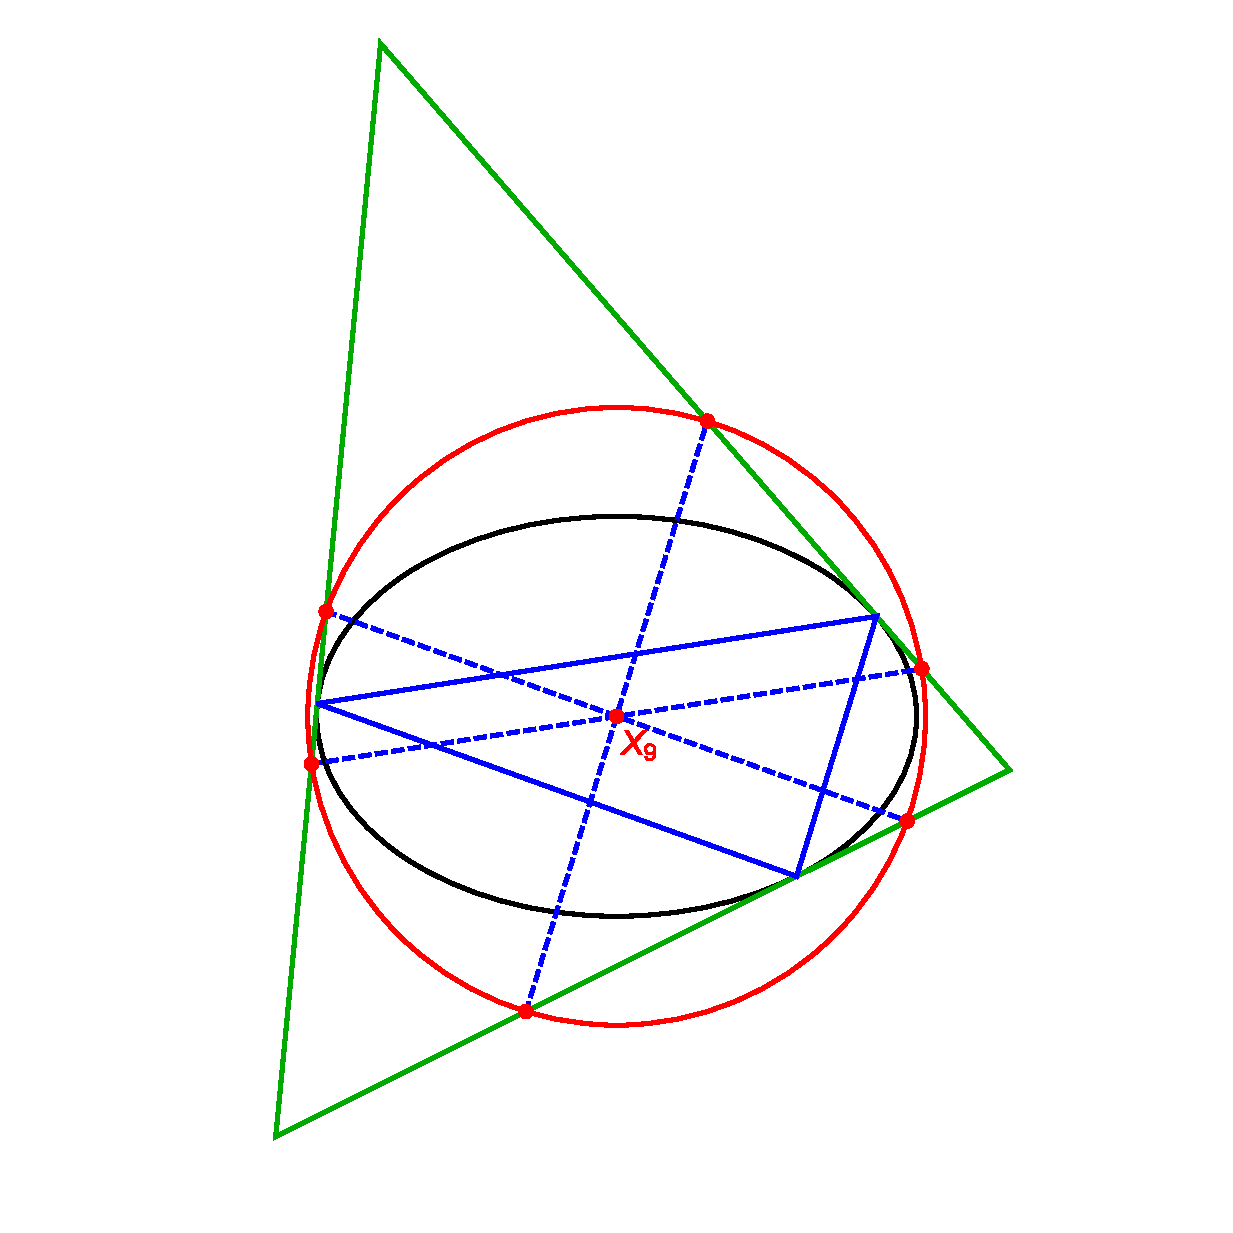
\includegraphics[width=.6\textwidth]{pics_03_130_exc_cosine_circle.eps}
    \caption{The cosine circle (red) of the excentral family (green) is stationary. It contains the 6 intersections of lines (dashed blue) through the common center (family's $X_6$ and billiard periodics' $X_9$) which are parallel to their orthic, i.e., sidelines of billiard 3 periodics. \href{https://youtu.be/CrOSI8d8qDc}{Video}}
    \label{fig:03-cos-circle}
\end{figure}

  
\subsection{Incircle Family}
The incircle family, shown in \cref{fig:03-n3-affine}(middle), is the Poncelet family in a CAP pair for which the caustic is a circle (let $r$ denote its radius). It follows immediately that the family's incenter $X_1$ is stationary. Let $a_e,b_e$ be the axes of the ellipse the family is inscribed in. Cayley yields $r=a_c=b_c=(a_e b_e)/(a_e+b_e)$. 

\begin{figure}
    \centering
    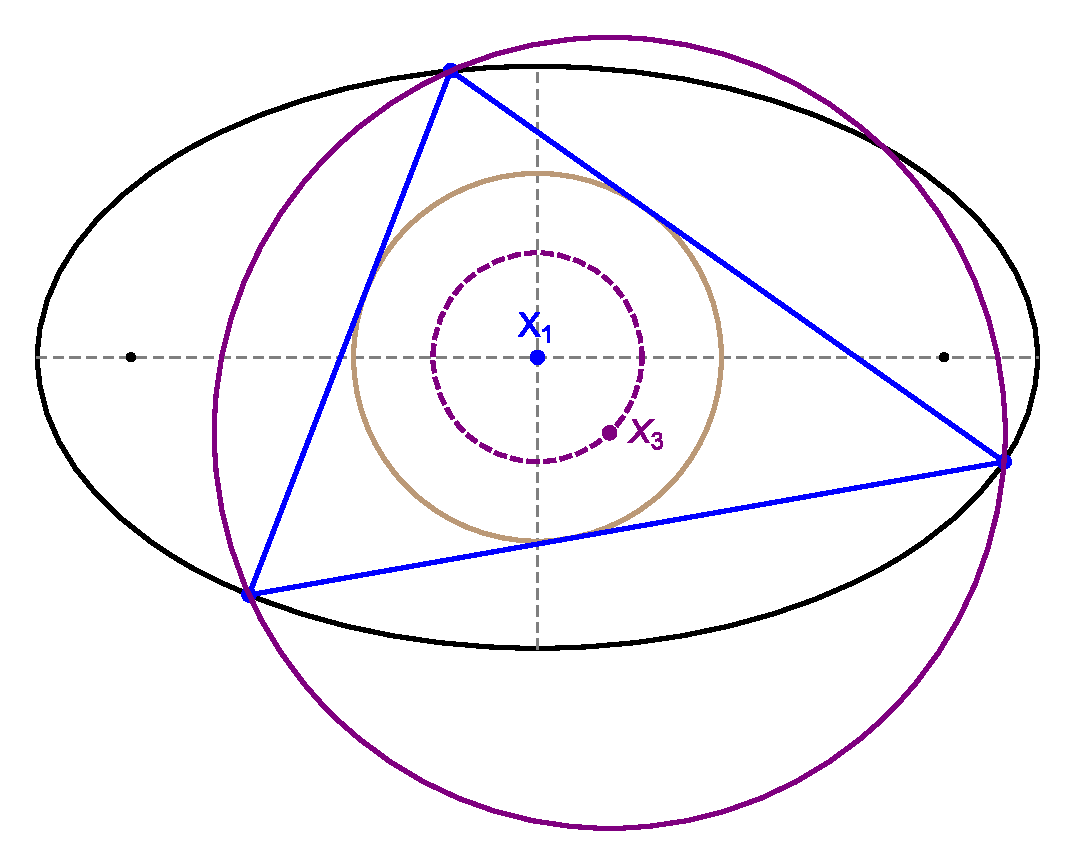
\includegraphics[width=.7\textwidth]{pics_03_160_incircle_circum.eps}
    \caption{A 3-periodic (blue) in the incircle family, and its fixed-radius circumcircle (purple). The locus of the circumcenter $X_3$ is a concentric circle (dashed purple). \href{https://bit.ly/3thddWK}{Live}}
    \label{fig:03-incircle-circum}
\end{figure}

As shown in \cref{fig:03-incircle-circum}:

\begin{proposition}
The incircle family has invariant circumradius given by $R=(a_e+b_e)/2$. Furthermore, the locus of its circumcenter $X_3$ is a circle of radius $d=R-b_e=a_e-R$ centered on the common center $O=X_1$.
\label{prop:n3-incircle-R}
\end{proposition}

\begin{proof}
Let $P_1=(x_1,y_1)$ be a first vertex of the incircle family. Using an explicit parametrization for $P_2$ and $P_3$, obtain via CAS the following coordinates for the moving circumcenter $X_3$:

{\scriptsize
\[
X_3=\frac{a_e-b_e}{2}\left[ - \,{\frac {x_1\, \left( -x_1^{2}
			\left( a_e+b_e \right) ^{2}+{a_e}^{2} b_e \left( 2\,a_e+b_e \right)  \right) }{ a_e
			\left(  \left( {a_e}^{2}-{b_e}^{2} \right) x_1^{2}+{a_e}^{2}{b_e}^{2}
			\right) }}
	 ,  {\frac { y_1\left( x_1^{2} \left( a_e+b_e
	 		\right) ^{2}-{a_e}^{2}{b_e}^{2} \right)}{b_e \left( {a_e}^{2}x_1^2+{b_e}^{2} \left( {a_e}^{2}-x_1^{2} \right)  \right) }}
	   \right]
 \]
 }

And circumradius $R=|P_1-X_3|=(a_e+b_e)/2$. Also obtain that the locus of $X_3$ is a circle concentric with the incircle and of radius $(a_e-b_e)/2$.
\end{proof}

Referring to \cref{eqn:03-sum-cos}: 

\begin{corollary}
The incircle family conserves its sum of cosines given by:
\[ \sum{\cos\theta_i}=1+\frac{r}{R}=\frac{{a_e}^2+4 {a_e}
   {b_e}+{b_e}^2}{({a_e}+{b_e})^2}\]
\label{cor:03-n3-inc-cos-sum}
\end{corollary}

\noindent \textbf{Affine image:} As \cref{fig:03-n3-affine}(middle) depicts, the incircle family can also be obtained from an affine image of billiard 3-periodics which sends the confocal caustic to a circle. As before, let $a,b$ be the semi-axes of its billiard ellipse pre-image.

\begin{lemma}
The confocal family is sent to the incircle family by scaling it along the major axis by an amount $s$ given by:

\[ s=\frac{b (\delta-c^2)}{a^3} \]

%\[ \lambda =\frac{(2a-r)\cdot r^3}{(a^2-r^2)\cdot (a-r)^2} \]
\label{lem:03-incircle-affine}
\end{lemma}

\begin{proof}
The scaled family will be inscribed in an ellipse with semi-axes $a_e = s a$, and $b_e =b$. Its caustic will be the circle $r=b_c$, where $b_c={b\left({a}^{2}-\delta\right)}/{c^2}$ is the confocal caustic minor axis given in \cref{prop:03-n3-caustic}. The Cayley condition for the incircle family imposes that $r=b_c=(a_e b_e)/(a_e + b_e)$, i.e., the result follows from solving $b_c = (s a b)/(s a + b)$ for $s$.

%The claim is obtained by imposing %$a_c^2-b_c^2=(s a)^2-b^2$ and solving %for $s^2$.
\end{proof}

\noindent Surprisingly:

\begin{proposition}
The sum of cosines conserved by the incircle family is identical to that conserved by billiard 3-periodics which are its affine pre-image.
\label{prop:03-incircle-same-sum-cos}
\end{proposition}

\begin{proof}
Let $s$ be the scaling along the major axis in \cref{lem:03-incircle-affine}. Plug $a_e=s a$ and $b_e=b$ into  \cref{cor:03-n3-inc-cos-sum}, subtract one (to obtain $r/R$ for the incircle family) and verify it yields the expression in \cref{thm:03-confocal-rovR}.
\end{proof}

\subsection{Circumcircle Family}

The circumcircle family, shown in \cref{fig:03-n3-affine}(right), is the Poncelet family in a CAP pair for which the outer ellipse is a circle (let $R$ denote its radius). It follows immediately that the family's circumcenter $X_3$ is stationary. Let $a',b'$ be the axes of its inellipse and $s_i$ the sidelengths. Cayley imposes $a'+b'=R$.

\begin{lemma}
Poncelet triangles in the circumcircle family are always acute.
\label{lem:03-circum-acute}
\end{lemma}

\begin{proof}
Since the stationary circumcenter $X_3$ is interior to the caustic caustic, it will be interior to circumcircle family triangles, and the result follows.
\end{proof}

\begin{proposition}
The circumcircle family conserves the sum of squared sidelengths. This is given by:

\[ \sum_{i=1}^3 s_i^2=4(a' + 2 b')(2 a' + b') \]
\end{proposition}

\begin{proof}
%\textcolor{red}{ronaldo}
CAS-assisted simplification from vertex parametrization given by \cref{eq:03-n3-conc-general}.
\end{proof}

\begin{proposition}
The circumcircle family conserves the product of its internal angle cosines. This is given by:
\[ \prod_{i=1}^3{\cos\theta_i}=\frac{a' b'}{2(a'+b')^2}=\frac{a' b'}{2 R^2}\]
\label{prop:03-circum-cos-prod}
\end{proposition}

\begin{proof}
CAS-assisted simplification from vertex parametrization.
\end{proof}

Recall the orthic triangle has vertices at the feet a triangle's altitudes. Let $R_h$ denote its circumradius. In , see \cite[Orthic Triangle, Eqn 7]{mw}, one finds the relation $R_h=R/2$. Therefore $R_h$ is invariant over the circumcircle family. Let $r_h$ denote the orthic's inradius. Referring to \cref{fig:03-circum-orthic}:

%Referring to Figure~\ref{fig:II-poristic} (left):

\begin{proposition}
Over the circumcircle family  $r_h$ is invariant and  given by $r_h=a' b'/(a'+b')$. 
\label{prop:03-circumcircle-rh}
\end{proposition}

\begin{proof}
In \cite[Orthic Triangle, Eqn. 5]{mw} one finds the relation  $r_h=2 R \prod_{i=1}^3{\cos\theta_i}$. Recalling $R=a'+b'$, substitution into \cref{prop:03-circum-cos-prod} yields the claim.
\end{proof}

\begin{figure}
    \centering
    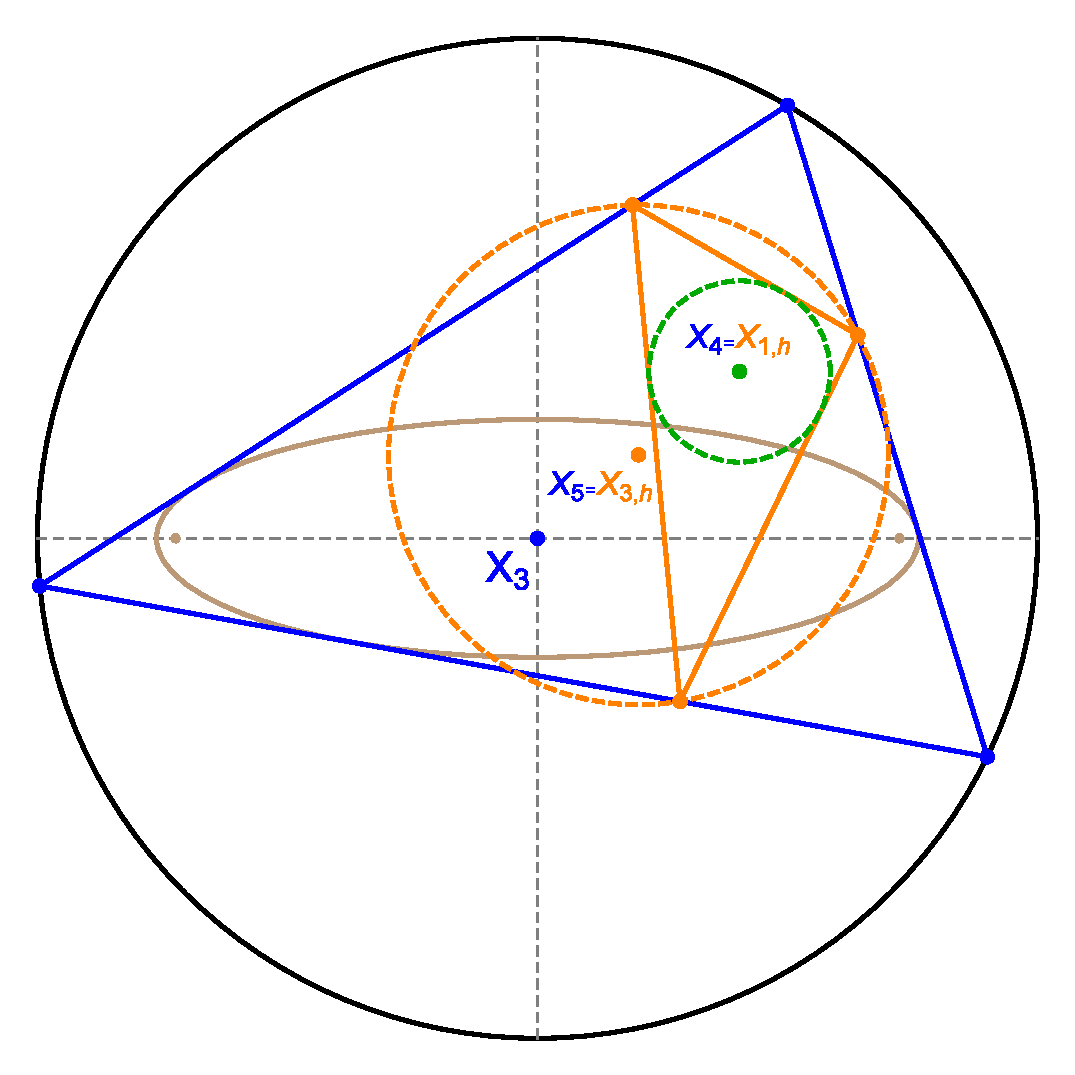
\includegraphics[width=.7\textwidth]{pics_03_140_circum_orthic.eps}
    \caption{A circumcircle family 3-periodic (blue) and its orthic triangle (orange). Over the family the orthic's circumcircle (dashed orange) and incircle (dashed green) have invariant radii. Also shown are their centers $X_{3,h}$ and $X_{1,h}$ which, for any reference triangle, correspond the nine-point center $X_5$ and orthocenter $X_1$. \href{https://youtu.be/wUu2iMesv3U}{Video}, \href{https://bit.ly/2PHJZma}{Live}}
    \label{fig:03-circum-orthic}
\end{figure}


Referring to  \cref{fig:03-circum-orthic}, it can be shown (see \cref{ex:03-circum-x5-locus}):

\begin{lemma}
Over the circumcircle family, the locus of the orthic circumcenter (i.e., the 9-point center $X_5$ of the family) is a circle concentric with the pair.
\label{lem:03-circum-x5-locus}
\end{lemma}

%Below we analyze a Poncelet family with fixed incircle and non-concentric fixed circumcircle, known as the ``poristic'' family. The previous result implies that the orthics derived from the circumcircle family can be regarded as a rigidly moving poristic family.

\noindent \textbf{Affine image:} As \cref{fig:03-n3-affine}(right) depicts, the circumcircle family can also be obtained from an affine image of billiard 3-periodics which sends the billiard ellipse with semi-axes $a,b$ to a circle with radius $R=b$. Therefore billiard 3-periodics are sent to the circumcircle family by scaling it along the major axis by an amount $s'={b/a}$. Therefore \cref{prop:03-n3-caustic} implies:

\begin{lemma}
The caustic semi-axes $a',b'$ of the circumcircle family which is the $s'$-affine image of the confocal family are given by:

\[ a'=\frac{b}{a}{a_c}=\frac{b(\delta-b^2)}{c^2},\;\;\;b'=b_c=\frac{b(a^2-\delta)}{c^2} \]
\label{lem:03-circumcircle-affine}
\end{lemma}

\noindent Note that the $s'$-affine image of billiard excentrals becomes a Poncelet family with fixed incircle; see \cref{fig:03-n3-affine}(right, dashed green triangles). We have seen above such a family conserves its sum of cosines. Suprisingly, the following invariant ``role reversal'' takes place:

\begin{proposition}
The sum of cosines conserved by billiard 3-periodics is the same as the one conserved by the $s'$-affine image of billiard excentrals. Furthermore product of cosines conserved by billiard excentrals is the same as the one conserved by the $s'$-affine image of billiard 3-periodics (circumcircle family). Furthermore, \label{prop:03-n3-role-reversal}
\end{proposition}

\begin{proof}
For the first statement it suffices to show that the $s'$-affine image of billiard excentrals has sides parallel to those of the $s$-image of billiard 3-periodics, i.e., the incircle family and use \cref{prop:03-incircle-same-sum-cos}.
\textcolor{red}{ronaldo consegue seguir: Vou pensar nisso. Ainda nao finalizei}
\end{proof}

\subsection{Homothetic Family}
 
\begin{figure}
    \centering
    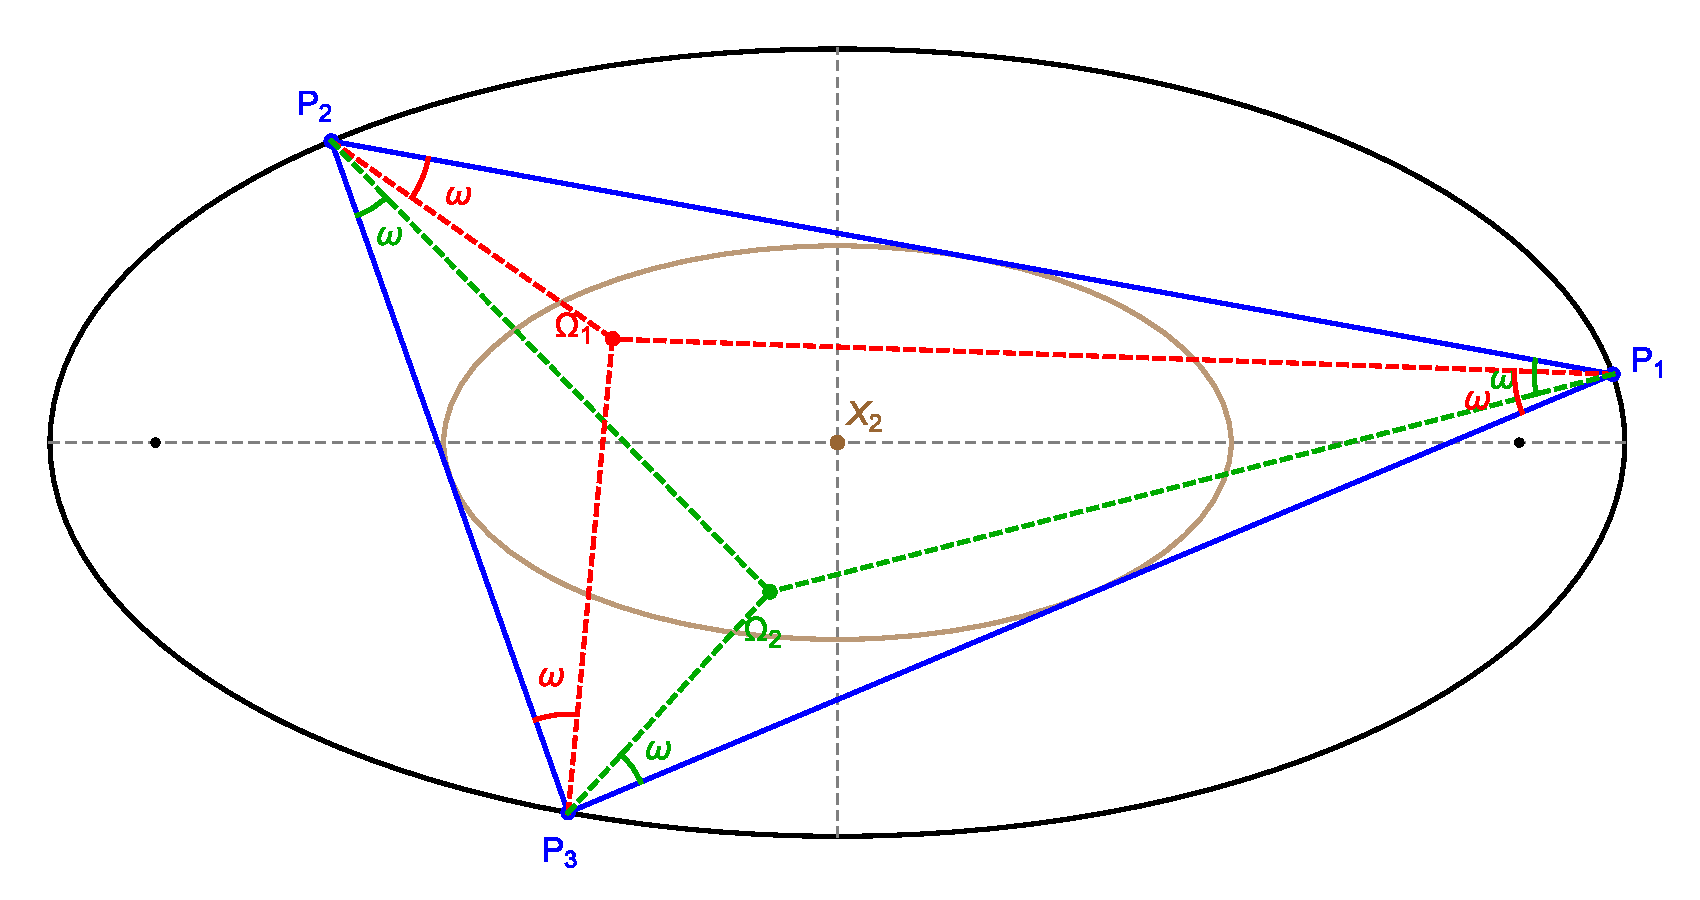
\includegraphics[width=\textwidth]{pics_03_150_n3_homothetic.eps}
    \caption{A 3-periodic (blue) interscribed between two homothetic ellipses (black, brown). Since this family is an affine image of one of equilaterals interscribed between two concentric circles, (i) the barycenter $X_2$ is stationary at the common center, and (ii) the area is conserved. Also conserved is (iii) the sum of squared sidelengths. (ii) and (iii) imply the Brocard angle $\omega$ is invariant. Also shown are the two (moving) the Brocard points $\Omega_1$ and $\Omega_2$. \href{https://youtu.be/2fvGd8wioZY}{Video}, \href{https://bit.ly/3aYnrVM}{Live}}
    \label{fig:03-homoth-brocard}
\end{figure}

The homothetic family, shown in \cref{fig:03-homoth-brocard}, is the Poncelet family in a CAP pair for which the outer and inner ellipse are homothetic to each other, i.e., $a_e = k a'$ and $b_e = k b'$, where $a_e,b_e$ and $a',b'$ are outer and inner ellipse semi-axes, respectively. Cayley imposes a homothecy ratio $k=1/2$.

\begin{proposition}
The barycenter $X_2$ is stationary at the common center and area $A$ is invariant and given by:
\[A= \frac{3\sqrt{3}}{4} a_e b_e \]
\end{proposition}

\begin{proof}
Consider an affine transformation that sends both outer and inner ellipse to a unit circle, e.g., by scaling the system along the major (resp. minor) axis by $1/a_e$ (resp. $1/b_e$). Uniquely amongst all triangle centers, the barycenter $X_2$ is invariant under affine transformations. By symmetry of the equilateral centroid, it will be identified with the center of the homothetic pair. Affine transformations preserve area ratios, so $A$ will be the the area of an equilateral triangle inscribed in a unit circle scaled by the inverse Jacobian $a_e b_e$. This completes the proof.
\end{proof}

Curiously, the homothetic family shares the following invariant with the circumcircle family:

\begin{proposition}
Over the homothetic family, the sum of squared sidelengths $s_i^2$ is invariant and given by:
	
\[ \sum_{i=1}^3 s_i^2=\frac{9}{2} \left(a_e^{2}+b_e^{2}\right) \]
\end{proposition}

The proof below was kindly contributed by  \cite{sergei2020-private-sidelengths}.

\begin{proof}
Invariant sum of squared sidelengths follows from the fact that the average of the harmonics of degree 1 and 2 over the group of rotations of order 3 is zero. Namely, consider a unit vector $v(\alpha)=(\cos \alpha, \sin \alpha)$ and a matrix $\mathcal{A}$ taking concentric circles to homothetic ellipses. Then $|\mathcal{A}v(\alpha)|^2$ is a trigonometric polynomial of degree 2. Average it over $\mathbb{Z}_3$ by adding $2\pi/3$ and $4\pi/3$ to $\alpha$. The result is independent of $\alpha$, as needed. The actual value is obtained via CAS simplification from vertex parametrization.
\end{proof}

Referring to \cref{fig:03-homoth-brocard}, recall the definition of a triangle's Brocard angle $\omega$, given in \cite[Brocard Angle]{mw}: sidelines $P_i P_{i+1}$ rotated about $P_i$ by some angle $\alpha$ will only concur (at the first Brocard point $\Omega_1$) if $\alpha=\omega$. A second, distinct Brocard point $\Omega_2$ exists if sidelines $P_i P_{i-1}$ are rotated about $P_{i}$ by $-\omega$.

A known relation appearing in \cite[Brocard Angle, Eqn. 2]{mw} is $\cot\omega=(\sum_{i=1}^3 s_i^2)/(4 A)$. Therefore:

\begin{corollary}
Over the homothetic family, the Brocard angle $\omega$ is invariant. Its cotangent is given by:
\[ \cot\omega=\frac{\sqrt{3}}{2} \frac{{a_e}^{2}+{b_e}^{2}}{a_e b_e} \]	
\end{corollary}

\begin{proof}
Direct calculations using the explicit parametrization of homothetic vertices.
\end{proof}

\noindent Another known relation valid for any triangle is $\cot\omega=\sum\cot\theta_i$:

\begin{corollary}
The homothetic family conserves the sum of its internal angle cotangents.
\end{corollary}

\subsection{Dual Family}

\begin{figure}
    \centering
    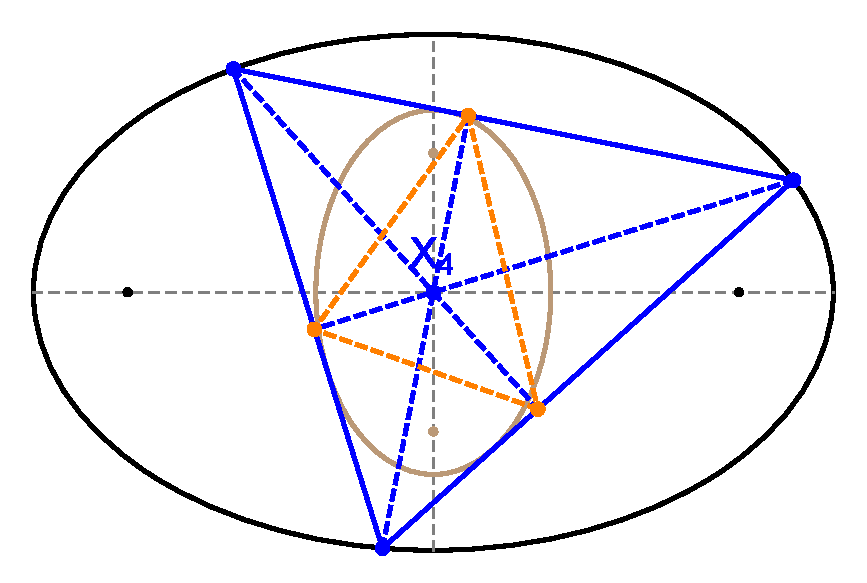
\includegraphics[width=.7\textwidth]{pics_03_120_dual_w_orthic.eps}
    \caption{A Dual family 3-periodic (blue) interscribed in a pair of ``dual'' ellipse (black, brown). Their aspect ratios are reciprocals of each other. No invariants have yet been detected for this family other than the fact that the orthocenter $X_4$ is stationary at the common center. Also shown is the orthic triangle (dashed orange) whose vertices lie at the feet of the altitudes (dashed blue). \href{https://bit.ly/337wTBS}{Live}}
    \label{fig:03-n3-dual}
\end{figure}

%\textcolor{red}{Quem e o dual: é aquele cuja caustica é anti-homotetica a externa, ou seja $a'/b'=b/a$}

The dual family, shown in \cref{fig:03-n3-dual}, is the Poncelet family in a CAP pair such that the outer and inner ellipses are ``duals'' curves of each other, i.e., tangents to one are sent to points on the other and vice-versa. For ellipses, this simply implies their aspect ratios $a_e/b_e$ and $a'/b'$ will be reciprocals of one another. Cayley yields $a'=\lambda b_e,\; b'=\lambda a_e$ and therefore $\lambda= a_e b_e/(a_e^2+b_e^2)$. Remarkably:

\begin{proposition}
The orthocenter $X_4$ of the dual family is stationary.
\end{proposition}

\begin{proof}
Follows directly from the vertex parametrization, see \cref{eq:03-n3-conc-general}.

In terms of the vertices of a triangle $A=[x_a,y_a]$, $B=[x_b,y_b]$, $C=[x_c,y_c]$ the orthocenter $X_4=[x_{4n}/A_4,y_{4n}/A_4]$ is given by the following rational functions 

\begin{align*}
    x_{4n}&=   \left(x_c-x_b\right) x_a\,y_a+ \left( 
 x_b\,y_b-x_c\,y_c \right) x_a+ \left( y_c-y_b \right) y_a^2+ \left( y_b^2-{y_c}^{2} \right) y_a\\
&+  x_cx_b\left( \,y_c- \,y_b)
 \right) +y_by_c( y_c-y_b) \\
 \\
 y_{4n}&=  \left(x_b-x_c\right) x_a^2+ \left( y_b-y_c \right) x_a\,y_a+ \left( x_c^2-x_b^2\right) x_a+ \left( -x_b\,y_b+x_c\,y_c \right) y_a\\
 &+x_b  x_c(x_b- \,x_c)+ y_b\,y_c(x_b-x_c) \\
 %
A_4&= \left(y_b-y_c \right) x_a+ \left( -x_b+x_c\right) y_a+x_b\,y_c-x_c\,y_b
\end{align*}

Therefore, using  the vertex parametrization, see \cref{eq:03-n3-conc-general}, and CAS the result follows by direct computations.
\end{proof}

Despite much searching, no invariant quantities have yet been found for this family.
